% !TeX root = ../../../main.tex
\begin{figure}[t!]
% \vspace{-4ex}
\ChTwoFloatContents
    {ch02:fig:model-overview}% label for whole figure
    {\caption{Overview of \ChTwoSmallCaps{Temporal-SCL}}}% caption for whole figure
    {%
        
        \subfigure[Encode patients at time step level]{%
            \label{ch02:fig:encoding}
            \centering
            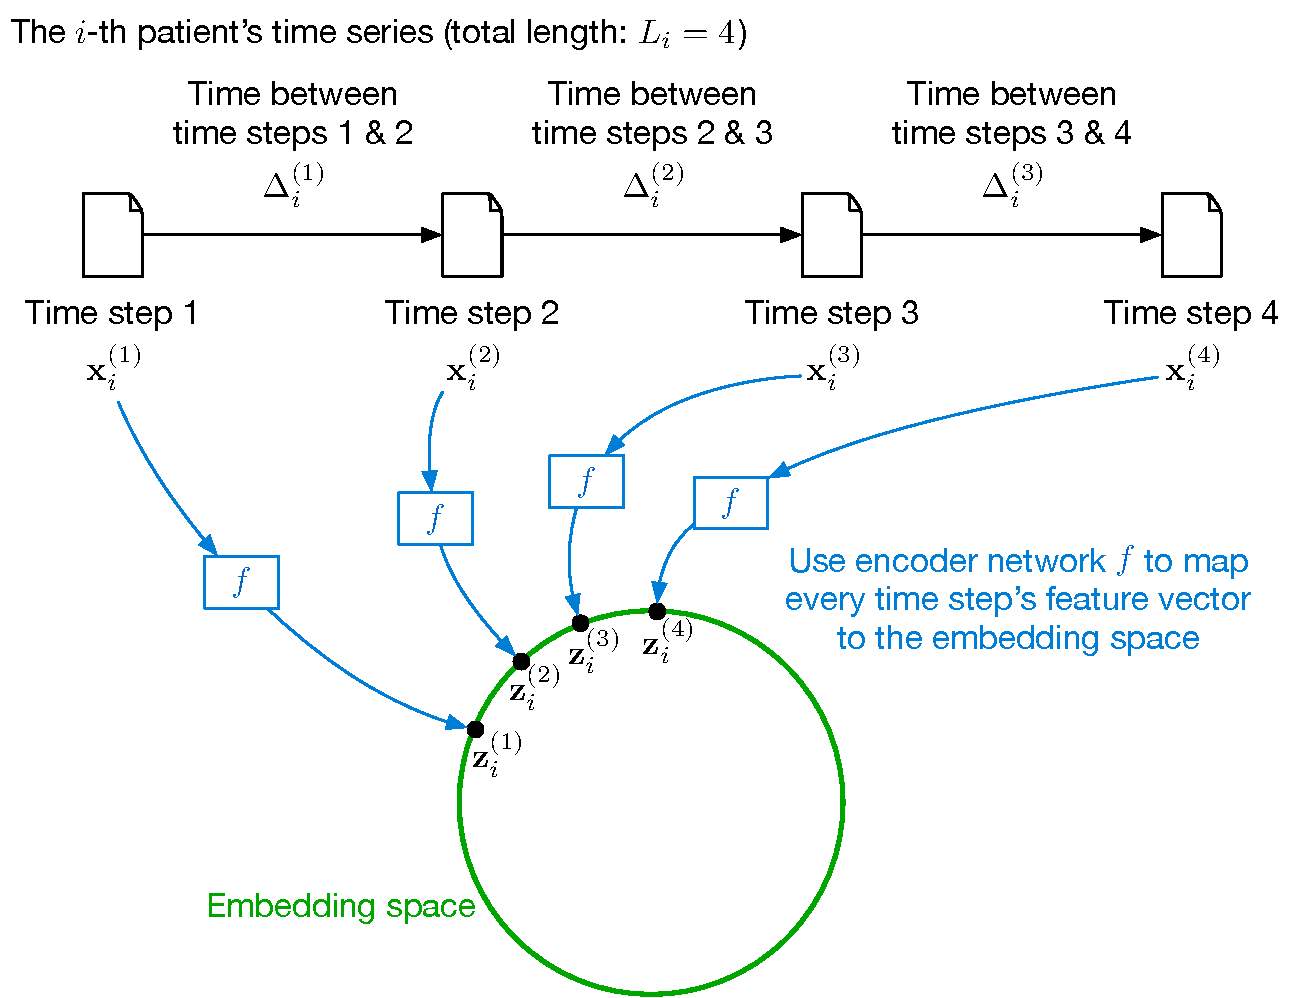
\includegraphics[width=0.48\linewidth,trim={6pt 0pt 6pt 6pt},clip]{Chapters/chapter-02/images/temporal-supervised-contrastive-learning-draft2-step1.pdf}
        } \\[.5em]
        \subfigure[Encourage temporal smoothness]{%
            \label{ch02:fig:temporal-smoothing}% label for this sub-figure
            \centering
            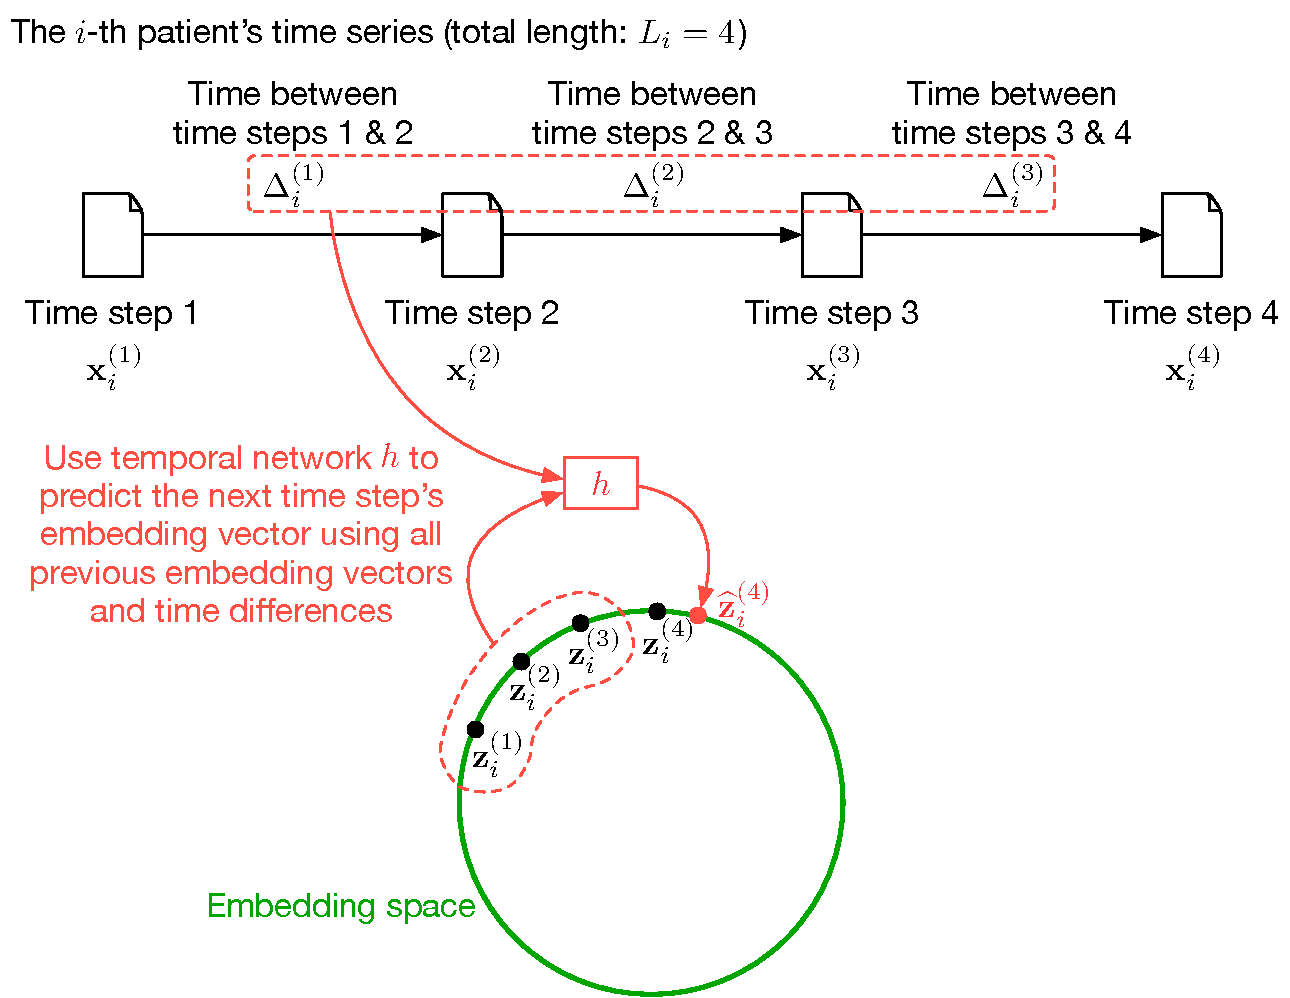
\includegraphics[width=0.48\linewidth,trim={6pt 0pt 6pt 6pt},clip]{Chapters/chapter-02/images/temporal-supervised-contrastive-learning-draft2-step2.pdf}
        } \\[0em]
        \subfigure[Predict using encoded representation]{%
            \label{ch02:fig:prediction}% label for this sub-figure
            \centering
            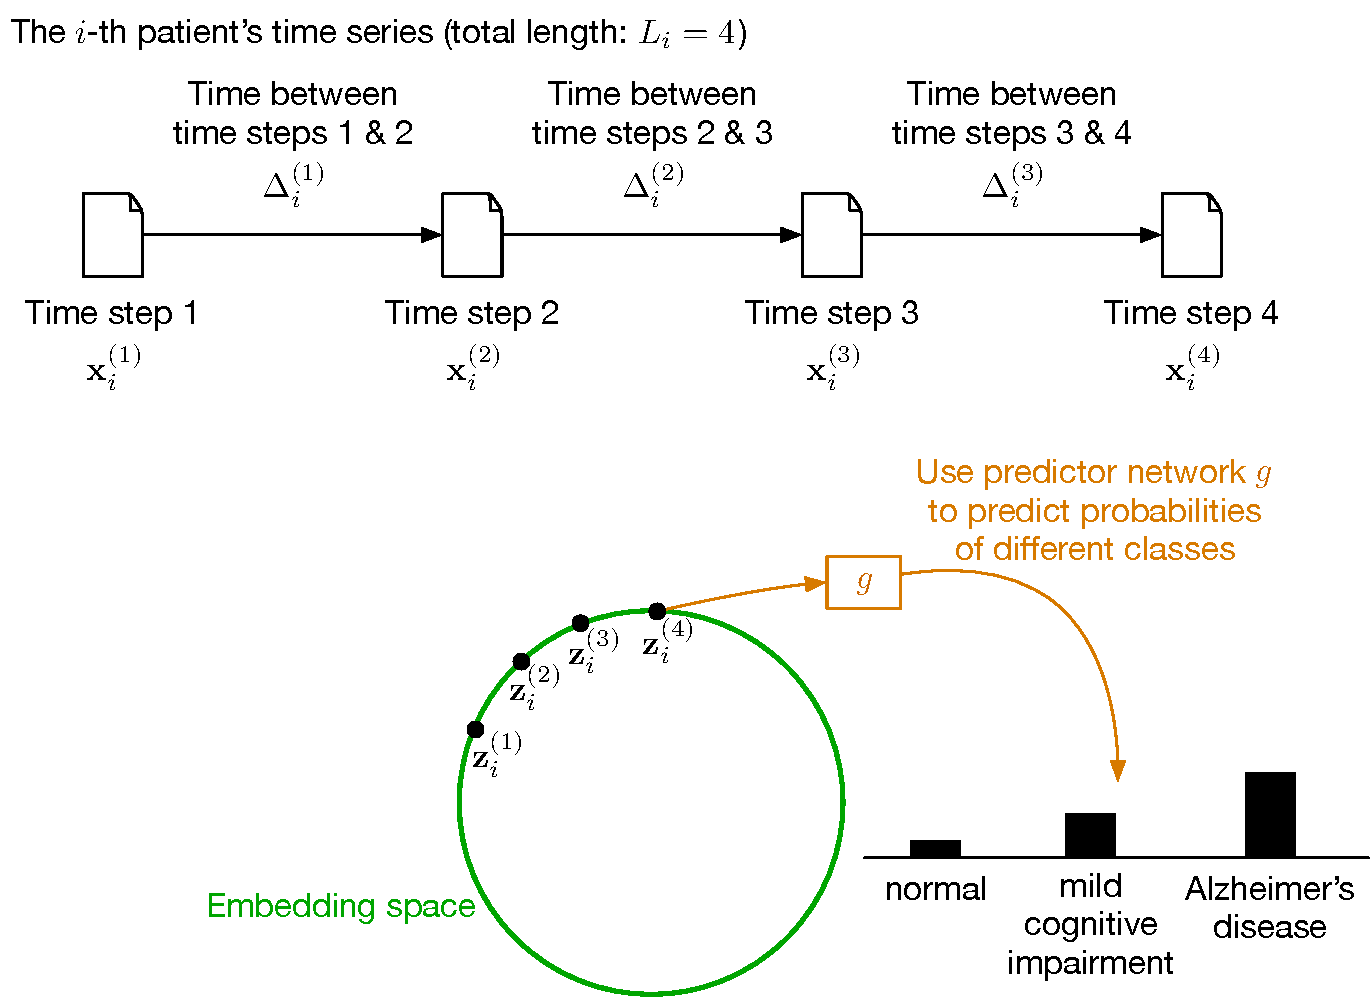
\includegraphics[width=0.48\linewidth,trim={6pt 0pt 6pt 21em},clip]{Chapters/chapter-02/images/temporal-supervised-contrastive-learning-draft2-step3-classification-version.pdf}
        }
        
    }
\end{figure}